\section{Implementation}

\subsection{Script: GetAndAnalyseAuditPolicies}
The basic idea was to implement the use case ''\nameref{UC01}'' separately from the use case ''\nameref{UC02}''. However, during the implementation it quickly became clear that these two use cases could be merged and did not have to be implemented separately. Therefore, both use cases were integrated into one script. The following describes how the two use cases were implemented.

\subsubsection{Result}\label{GetAndAnalyseAuditPoliciesResult}
Both Use Cases were implemented together in one script. The script follows the following schedule:
\begin{itemize}
    \item Reading and caching of the RSoP
    \item Verification that all defined audit policies are in place
    \item Verification that all defined audit policies are correctly configured
    \item Check if ''Audit: Force audit policy subcategory settings (Windows Vista or later) to override audit policy category settings'' is enabled in registry to prevent conflicts between similar settings
    \item Check if Sysmon is installed and running as a service
    \item Check whether CAPI2 is enabled
\end{itemize}
Each result of the individual steps is then collected in a common XML file. Finally, the environment and files that are no longer needed are deleted, so that only the result XML is available for further processing. A result could possibly look like the following listing:
\begin{lstlisting}[caption=Example Result Audit Policy Analysis, language=xml]
<?xml version="1.0"?>
<AuditPolicies>
    <AuditRegistry>NotConfigured</AuditRegistry>
    <AuditProcessTermination>NotConfigured</AuditProcessTermination>
    <AuditProcessCreation>NotConfigured</AuditProcessCreation>
    <AuditFilteringPlatformConnection>NotConfigured</AuditFilteringPlatformConnection>
    <AuditKernelObject>NotConfigured</AuditKernelObject>
    <AuditNonSensitivePrivilegeUse>NotConfigured</AuditNonSensitivePrivilegeUse>
    <AuditHandleManipulation>NotConfigured</AuditHandleManipulation>
    <AuditDetailedFileShare>NotConfigured</AuditDetailedFileShare>
    <AuditFileSystem>Success</AuditFileSystem>
    <AuditKerberosAuthenticationService>Failure</AuditKerberosAuthenticationService>
    <AuditKerberosServiceTicketOperations>Success</AuditKerberosServiceTicketOperations>
    <AuditLogoff>SuccessAndFailure</AuditLogoff>
    <AuditFileShare>NoAuditing</AuditFileShare>
    <AuditSAM>SuccessAndFailure</AuditSAM>
    <AuditSensitivePrivilegeUse>SuccessAndFailure</AuditSensitivePrivilegeUse>
    <AuditUserAccountManagement>SuccessAndFailure</AuditUserAccountManagement>
    <AuditSecurityGroupManagement>SuccessAndFailure</AuditSecurityGroupManagement>
    <AuditSpecialLogon>SuccessAndFailure</AuditSpecialLogon>
    <AuditLogon>SuccessAndFailure</AuditLogon>
    <AuditMPSSVCRule-LevelPolicyChange>Failure</AuditMPSSVCRule-LevelPolicyChange>
    <ForceAuditPolicySubcategory>Enabled</ForceAuditPolicySubcategory>
    <Sysmon>Installed</Sysmon>
    <CAPI2>EnabledGoodLogSize</CAPI2>
</AuditPolicies>
\end{lstlisting}

\subsubsection{Approach}
\paragraph{Read Resultant Set of Policies} \ \\
Research was done to read the corresponding audit policy configurations from the system. At the beginning, the approach was to read the required configurations using the command \lstinline|auditpol|. \cite{auditpol} This command can be used to read out and manipulate the currently valid information on the audit policies. However, the manipulation of the audit policies is not necessary within the tool and can be ignored. The command provides exactly the information needed to fulfill this use case:
\begin{lstlisting}[caption=auditpol, language=PowerShell]
PS C:\Windows\system32> auditpol /get /category:Logon/Logoff
System audit policy
Category/Subcategory                        Setting
Logon/Logoff
    Logon                                   Success and Failure
    Logoff                                  Success and Failure
    Account Lockout                         No Auditing
    IPsec Main Mode                         No Auditing
    IPsec Quick Mode                        No Auditing
    IPsec Extended Mode                     No Auditing
    Special Logon                           Success and Failure
    Other Logon/Logoff Events               No Auditing
    Network Policy Server                   No Auditing
    User / Device Claims                    No Auditing
    Group Membership                        No Auditing
\end{lstlisting}
Unfortunately, this output is not very ideal for a suitable further processing and analysis of the current configuration. The return value of the command is an ordinary array filled with corresponding strings and therefore the complete array should have been checked for correct content by string comparisons. Furthermore, the command \lstinline|auditpol| does not offer the possibility of remote configuration with regard to an extension of the tool to a whole fleet of computers. For this reason, the idea of building the tool on the basis of this command was rejected.
\\\\
Further research has shown that Microsoft provides a RSoP \cite{RSoP} for reading audit policies. This can also be accessed via a PowerShell command. Microsoft offers the command \lstinline|Get-GPResultantSetOfPolicy| \cite{GetGPResultantSetOfPolicy} for this purpose. This command can be used to generate an XML-based report of the currently valid GPOs. Since traversing an XML-based file via PowerShell proves to be very simple, this variant is preferable to the \lstinline|auditpol| command. After a short test, it quickly became clear that the generated XML provides all necessary information for the further analysis.


\paragraph{Analyse Audit Policies} \ \\
The current configuration of the system's audit policies is then to be evaluated from the temporarily cached file. The basis for this provides the section ''\ref{Correlation} \nameref{Correlation}'' based on ''\ref{JPCertStudy} \nameref{JPCertStudy}''.

\clearpage 

\subsubsection{Implementation}
This section describes the implementation of \lstinline|GetAndCheckAuditPolicies| in detail. For this purpose, the following is referred to in the section \ref{GetAndAnalyseAuditPoliciesResult} \nameref{GetAndAnalyseAuditPoliciesResult} described schedule.
\\\\
The first step is to read the RSoP from the local system with the command \lstinline|Get-GPResultantSetOfPolicy|. The XML that is retrieved is then temporarily cached in the execution path of the script and read in again for further processing.
\begin{lstlisting}[caption=Get-GPResultantSetOfPolicy, language=PowerShell]
$currentPath = (Resolve-Path .\).Path
$pathRSOPXML = $currentPath + "\LocalUserAndComputerReport.xml"
Get-GPResultantSetOfPolicy -ReportType Xml -Path  $pathRSOPXML | Out-Null;
[xml]$rsopResult = Get-Content $pathRSOPXML;
\end{lstlisting}
\vspace{1cm}
\begin{multicols}{2}
    \ \\\\\\ \
    The generated XML is an extraction of the GPOs and contains only the configurations set from them.
    Afterwards the analisis begins and the entries are searched in the XML file, in which the required configurations for the ''Advanced Audit Policies'' are stored (see figure \ref{fig:AdvancedAuditPolicies}).
    \begin{figure}[H]
        \centering
        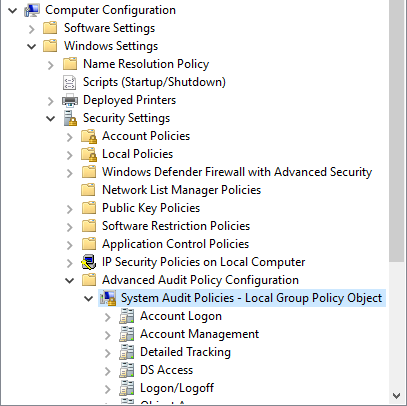
\includegraphics[width=0.7\linewidth]{assets/GetAndCheckAuditPolicies/advancedauditpolicies.png}
        \caption{GPO - Advanced Audit Policies}\label{fig:AdvancedAuditPolicies}
    \end{figure}
\end{multicols}
The first step of the analysis is to search for missing configurations. The system iterates over the queried \lstinline|AuditSettings| and searches for missing configurations.
\begin{lstlisting}[caption=GetAndCheckAuditPolicies: Search missing configurations, language=PowerShell]
$auditSettings = $rsopResult.Rsop.ComputerResults.ExtensionData.Extension.AuditSetting

foreach($auditSettingSubcategoryName in $auditSettingSubcategoryNames) {
    if($auditSettings.SubcategoryName -notcontains $auditSettingSubcategoryName){
        # Write to XML
    }
}
\end{lstlisting}

\clearpage
After checking for missing configurations the set settings are checked for correctness according to \nameref{JPCertStudy}.

\begin{lstlisting}[caption=, language=PowerShell]
foreach($auditSetting in $auditSettings) {
    # check if $auditSetting is not Null
    if($auditSetting) { 
        # try to get audit setting value, if not No Auditing is configured system will throw exception -> set value to 0 for NoAuditing
        try {
            $auditSettingValue = $auditSetting.SettingValue 
        }
        catch {
            $auditSettingValue = 0
        }
        $auditSubcategoryName = $auditSetting.SubcategoryName 
        switch ($auditSettingValue) {
            NoAuditing {  
                # Write SubcategoryName as tag with value  'NoAuditing' to XML
                continue
            }
            Success {
                # Write SubcategoryName as tag with value 'Success' to XML
                continue
            } 
            Failure {
                # Write SubcategoryName as tag with value 'Failure' to XML
                continue
            }
            SuccessAndFailure {
                # Write SubcategoryName as tag with value 'SuccessAndFailure' to XML
                continue
            }
            Default { continue }
        }
    }    
}
\end{lstlisting}
After checking the audit policies which can be configured through ''Advanced Audit Policies'' the next step is to verify if the setting ''Audit: Force audit policy subcategory settings (Windows Vista or later) to override audit policy category settings'' is enabled as considered in section ''\ref{DomainModelAuditPolicy} \nameref{DomainModelAuditPolicy}''. This had to be solved via the registry, because this information is not available in the RSoP.
\begin{lstlisting}[caption=Function IsForceAuditPoliySubcategoryEnabeled, language=PowerShell]
Function IsForceAuditPoliySubcategoryEnabeled {
    $path = "HKLM:\System\CurrentControlSet\Control\Lsa"
    $name = "SCENoApplyLegacyAuditPolicy"
    try {
        $auditPoliySubcategoryKey = Get-ItemProperty -Path $path -Name $name -ErrorAction Stop
        if ($auditPoliySubcategoryKey.SCENoApplyLegacyAuditPolicy -eq 1) {
            return "Enabled"
        } else {
            return "Disabled"
        }
    }
    catch {
        return "NotDefined"
    }
}
\end{lstlisting}
The next step is to check if Sysmon as a service (also not contained in the RSoP) is installed and if so is it running or not. 
\begin{lstlisting}[caption=Function IsSysmonInstalled, language=PowerShell]
Function IsSysmonInstalled {
    $service = $null

    try {
        $service = Get-Service -Name Sysmon*
    } catch {
        return "NotInstalled"
    }
    
    if ($service.Status -ne "Running") {
        return "InstalledNotRunning"
    } else {
        return "Installed"
    }
}
\end{lstlisting}
As a last step the script is checking whether CAPI2 is enabled and has the right minimum log size of 4MB. Unfortunately, this information is also not available via the RSoP. Therefore the command \lstinline|wevtutil| is used to query CAPI2 in the event log. The reason for this is that CAPI2 can only be enabled via the Event Viewer. \cite{CAPI2} 
\begin{lstlisting}[caption=Function IsCAPI2Enabled, language=PowerShell]
Function IsCAPI2Enabled {
    [xml]$capi2 = wevtutil gl Microsoft-Windows-CAPI2/Operational /f:xml
    $capi2Enabled = $capi2.channel.enabled
    $capi2LogSize = $capi2.channel.logging.maxsize -as [int]
    if ($capi2Enabled -eq "true" -and $capi2LogSize -ge 4194304) {
        return "EnabledGoodLogSize"
    } elseif ($capi2Enabled -eq "true" -and $capi2LogSize -lt 4194304) {
        return "EnabledBadLogSize"
    } else {
        return "Disabled"
    }
}    
\end{lstlisting}
At the end of the script all temporary files are removed.
\clearpage

\subsection{Script: GetAndCompareLogs}
This section describes the implementation of the ''\nameref{UC03}'' as well as ''\nameref{UC04}''. Both use cases were fulfilled in the PowerShell script ''GetAndCompareLogs''. Here is a description how the use cases were implemented.

\subsubsection{Result} \label{ResultSetGetAndCompareLogs}
The script ''GetAndCompareLogs'', where both use cases were implement, runs as follows:
\begin{itemize}
    \item Reading and caching the Event Logs ''System'' \& ''Security''
    \item Filter cached Logs by EventID, group EventIDs that occur more than once. Found EventIDs are exported as ''CSV''
    \item Checking and caching whether a list of EventIDs from ''Application and Service'' Logs can be read out
    \item Export result set of found EventIDs as ''CSV''
    \item Import list of found Event Logs and compare it with the predefined checklist
    \item Result of the comparison is written into an ''XML'' file
    \item Import and compare found Application and Service Logs with predefined checklist
    \item Result of the comparison is written into the same ''XML'' as before
\end{itemize}
The now no longer needed CSV files are deleted. The XML with the result set is now available for any further processing.  A result could possibly look like the following listing:
\begin{lstlisting}[caption=Example Result Audit Policy Analysis, language=xml]
    <?xml version="1.0"?>
    <Logs>
        <EventLogsID>
            <6>present</6>
            <21>missing</21>
            <24>missing</24>
            <102>missing</102>
            <104>missing</104>
            <106>missing</106>
            <201>missing</201>
            <4624>present</4624>
            <4634>present</4634>
            <4648>present</4648>
            <4656>present</4656>
            ...
        </EventLogsID>
        <AppAndServID>
            <106>present</106>
            <200>present</200>
            <129>present</129>
            <201>present</201>
            <102>present</102>
            <6>missing</6>
            <169>missing</169>
            <21>present</21>
            <24>present</24>
        </AppAndServID>
    </Logs>
\end{lstlisting}


\subsubsection{Approach}
\paragraph{Get Event Logs}\ \\
After research was done on how to read out the Event Logs ''System'' and ''Security'' the desicon was made to use to PowerShell command\lstinline|Get-EventLog| \cite{Get-EventLogs}. This command allows to read out the whole EventLog by the LogName or also to search after a specific EventID. The first approach was to search for each EventID individually. The EventIDs to search for were taken from the JPCERT/CC Appendix B in the ''Detecting Lateral Movement through Tracking Event Logs'' report. \cite{JPCERTDetectingLateralMovement}. The script run successfully, but the runtime was not practicable. It took over 5 minutes to search for all EventIDs in an Event Log of the size of about 37 000 Logs, or  in other words 300 Kilobyte (KB). The developers than started to calculate the worst case scenario, in this case the worst case scenario is that none of the searched EventIDs is found in the EventLog. There are \textit{n} EventIDs in the checklist and \textit{m} entries in the EventLogs, if no EventID is found, every entry is called \textit{m} times. That results in O(n*m). The developers decided to cache the Event Logs, reducing the runtime to O(m). The cached Logs are then grouped into EventIDs and export into a ''CSV'' file. \ \\
\ \\
To read out the ''Application and Service'' Logs we can not use Get-EventLog. The first approach used the \lstinline|Get-WinEvent| \cite{Get-WinEvent} command. The logic stayed the same, read out all events, group and export them into a 'CSV' file. Unfortunately the Get-WinEvent is very slow, it took over 10 minutes to read out just under 6000 logs.
The developers found an other, much quicker command called \lstinline|wevtutil| \cite{wevtutil}. Unfortunately it is not quite simple to read out all Logs, for that reason each EventID will be searched if it appeared. Unlike Get-EventLog, this is not a problem because the command is faster, the EventIDs are more likely to occur and the amount of Logs is smaller. On the testing environment with a machine with 4 Gigabyte (GB) Ram and an Intel Xeon E5 with 2 cores it took about 10 seconds to check for 9 EventIDs in 15 000 Log entries. If and EventID was found it was added to an ArrayList, after all IDs are checked the file is exported as a 'CSV'.
\paragraph{Analyse Found Event Logs} \ \\
To analyse the occurred EventIDs the two generated ''CSV'' files are imported into the PowerShell script. The respective checklists, which are based on the \nameref{JPCertStudy}, are embedded in the script. Each id from the checklist is checked if it is present in the respective CSV file. Is this the case, the id is added to the XML-file and marked as present. Did the id no occur in the it will be added and marked as missing. The file looks like the example in ''\nameref{ResultSetGetAndCompareLogs}'' shown.
\clearpage

\subsubsection{Implementation}
This section describes the implementation of \lstinline|GetAndCompareLogs| in detail. For this purpose, the following is referred to in the section ''\ref{ResultSetGetAndCompareLogs} \nameref{ResultSetGetAndCompareLogs}'' described schedule.
\\\\
The first step is to read out the ''System'' and ''Security'' Logs. To achieve this goal the command \lstinline|Get-EventLog| is used in the first part of the function \lstinline|GetEventLogsAndExport|. \begin{description}
    \item[Note] The code has been adapted for better readability and easier understanding
    \end{description}
\begin{lstlisting}[caption=Function GetEventLogsAndExport Part 1, language=PowerShell]
    $logNames = @("System", "Security")
    $eventLogs = New-Object System.Collections.ArrayList

    Function GetEventLogsAndExport{
        foreach($log in $logNames){
        $eventLogs += Get-EventLog -LogName $log
        }
    ...
\end{lstlisting}
The second part of the function filters the EventIDs from the chaced logs. Subsequently, multiple EventIDs are grouped together.
\begin{lstlisting}[caption=Function GetEventLogsAndExport Part 2, language=PowerShell]
    $currentFolder = (Resolve-Path .\).Path
    $exportEventLogsIntoCSV=$currentFolder + "\myeventlogs.csv"

    $eventLogs| Select EventID -Unique |Export-CSV $exportEventLogsIntoCSV -NoTypeInfo -Encoding UTF8
    }
\end{lstlisting}
After the export the function \lstinline|GetApplicationAndServiceLogs| is called. As before, the function is divided into two parts, first how to get the data. The same procedure is used three times, for the ''TaskScheduler'', ''WindowsRemoteManagement'' and ''LocalSessionManager''. Due to the fact that the code is very similar it is only shown once. To search for the EventIDs  \lstinline|wevtutil| is used.
\begin{lstlisting}[caption=Function GetApplicationAndServiceLogs Part 1, language=PowerShell]
    $appAndServLogs = New-Object System.Collections.ArrayList
    $idsForTaskScheduler = ("106", "200", "129", "201", ...

    $appAndServLogs += "EventID"

    Function GetApplicationAndServiceLogs{
    
    foreach($id in $idsForTaskScheduler){
    if(wevtutil qe Microsoft-Windows-TaskScheduler/Operational /q:"*[System[(EventID="$id" )]]" /uni:false /f:text){
        $appAndServLogs += $id
         }
    }
    ...
\end{lstlisting}
\clearpage
After all three Logs were checked and all found EventIDs were added, the information is exported into a ''CSV''-file.
\begin{lstlisting}[caption=Function GetApplicationAndServiceLogs Part 2, language=PowerShell]
    $exportApplicationAndServiceLogsIntoCSV = $currentFolder + "\myapplicationandservicelogs.csv"

    $appAndServLogs | Out-File -FilePath $exportApplicationAndServiceLogsIntoCSV
    }
\end{lstlisting}
The next point on the list is importing the found ''EventLogs'' and ''Service And Application'' Logs. Due to the similarity we only show one code.
\begin{lstlisting}[caption=Function ImportCompareExport, language=PowerShell]
    
    $eventLogIdsToCheck = (6, 21, 24, 102, 104, 106, 129, ...

    # Create XML "resultOfEventLogs.xml"

    $importEventLogs = $exportEventLogsIntoCSV
    $myEventLogs = Import-Csv $importEventLogs -Encoding UTF8

    Function ImportCompareExport{
        foreach($id in $eventLogIdsToCheck){
           if($myEventLogs | where {$_.EventID -eq $id}){
            # Write to XML with value "present"
                }
                else{
                    # Write to XML with value "missing"
                }
        }
    }
    # Close XML
\end{lstlisting}
The same happens with the ''App and Service'' Logs in the \lstinline|GetApplicationAndServiceLogs| function. At the end all temporary files are deleted.
\clearpage
\subsection{Script: Visualize}
In this script the ''\nameref{UC05}'' is implemented, here the description how it was done.
\subsubsection{Result} \label{resultVisualize}
The script ''\nameref{UC05}'' runs as follows:
\begin{itemize}
    \item Create Protable Document Format (PDF) at given folder and ''open'' it
    \item Import audit policies and compare them to a given checklist, result is written and visualized in a table
    \item Check which attack tool categories can be detected with the current audit guidelines and which cannot
    \item Import the found EventLogs and check if the important EventIDs, according to JPCERT/CC, are found
    \item ''Close'' PDF-document
\end{itemize}
The resulting PDF looks something like this: \ \\
\ \\
\textbf{AuditPolicies}
\begin{table}[H]
    \centering
    \begin{tabular}{| p{4.5cm} |  p{4cm} | p{4cm} | p{2.5cm}|} \hline
        Aduit Name & Target & Actual & Prio\\ \hline
        AuditNonSensitivePrivilege & SuccessAndFailure &\cellcolor{green} SuccessAndFailure & High\\ \hline
        AuditProcessTermination & Success &\cellcolor{darkgreen} SuccessAndFailure & Medium \\ \hline
        AuditSAM & SuccessAndFailure &\cellcolor{red} NotConfigured & Low\\ \hline
        ... & ... & ... &\\ \hline
    \end{tabular}
\end{table}\ \\
With this policies it is possible to detect X out of 14 attack categories \ \\
The following attack categories cannot be detected with certainty: \\
... \ \\
\ \\
\textbf{WindowsLogs}
\begin{table}[H]
    \centering
    \begin{tabular}{| p{8cm} |  p{8cm} |} \hline
        EventID6 & present \\ \hline
        EventID104 & missing \\ \hline
        ... & ... \\ \hline
    \end{tabular}
\end{table}
\subsubsection{Approach}
At first, the developers toyed with the idea to use ''PowerBI'' \cite{PowerBI}, like Jessica Payne uses it in ''WEFFELS''. But after a short tryout they decided that the tool was too overpowered for their purpose. Also did they not like that the user would have to install a third-party tool to analyse his data. The Dynamic Link Library (DLL) ''iTextSharp'', originally a C\# library, allows to generate a PDF directly from the code, which can also be used in PowerShell. This variant is not very versatile and it is difficult to create an appealing design, but it is enough for now. 

\subsubsection{Implementation}
This section describes the implementation of \lstinline|Display missing or wrong system configuration| in detail. For this purpose, the following is referred to in the section ''\ref{resultVisualize} \nameref{resultVisualize}'' described schedule. \\\\
The iTextSharp.dll and the functions from \lstinline|PowerShell-PDF| \cite{PowerShell-PDF} were imported. The first step is to create a PDF-document and ''open'' it. For this purpose the function \lstinline|OpenPDF| was created:
\begin{lstlisting}[caption=Function OpenPDF, language=PowerShell]
function OpenPDF{
    $pdf = New-Object iTextSharp.text.Document 
    New-PDF -Document $pdf -File #export path
    $pdf.Open()
   }
\end{lstlisting}
The function \lstinline|WriteAuditPolicies| then compares the found audit policies and display the ones who are incorrectly. It will call two other functions, \lstinline|CreateAddCellWithColor| and \lstinline|CreateAddCell|.
\begin{lstlisting}[caption=Functions WriteAuditPolicies \& CreateAddCellWithColor \& CreateAddCell, language=PowerShell]
function WriteAuditPolicies{
    $auditChecklist = @{AuditLogon = @("Success", "Medium"; ...)}
    $incorrectAudits = @() # will be returned for later use
    [xml] auditXml = Get-Content $auditPath
    $myAudits = $auditXml.AuditPolicies.ChildNodes
    foreach ($audit in $myAudits) {
        $localName = $audit.LocalName
        CreateAddCell $localName # Display auditname into cell

        $checkaudit = $auditChecklist[$localName]
        $checkauditvalue = $checkaudit[0] # Correct setting
        $checkauditprio = $checkaudit[1] # Priority of audit

        if ($audit.InnerXml -eq $checkauditvalue) { # Checks if audit values are equal
            CreateAddCell $checkauditvalue # Displays correct audit value
            CreateAddCellWithColor $audit.InnerXml 0 255 0 
            # Displays actual audit value into cell, color green  
        }
        elseif ($audit.InnerXml.startswith("Succ") #checks if audit is ''overpowered''
        -and $checkauditvalue -eq "Success") {
            CreateAddCell $checkauditvalue # Displays correct audit value
            CreateAddCellWithColor $audit.InnerXml 0 106 0 
            # Displays actual audit value into cell, color darkgreen
        }
        else { #audit is wrong
            CreateAddCell $checkauditvalue # Displays correct audit value
            CreateAddCellWithColor $audit.InnerXml 255 0 0 
            #Displays actual audit value into cell, color red
            $incorrectAudits += $audit.LocalName
        }
        CreateAddCell $checkauditprio # Displays audit priority into cell
    }
    return $incorrectAudits
}






function CreateAddCellWithColor($content, $R, $G, $B) {
    # Create iTextSharp.text.Paragraph and add content
    # Create  iTextSharp.text.pdf.PdfPCell with paragraph and set backgroundcolor $R $G $B
    # Add Cell to Table
    }

function CreateAddCell($content) {
        # Create iTextSharp.text.Paragraph and add content
        # Create  iTextSharp.text.pdf.PdfPCell with paragraph
        # Add Cell to Table
}
\end{lstlisting}
Now that the ''Import audit policies and compare them to a given checklist,result is written and visualized in a table'' is done, it is possible to check which attack tool categories can be detected with the current audit settings. For that purpose the function \lstinline|ToolsCanBeDetected| was created. This function relies on the return of the \$incorrectAudits.
\begin{lstlisting}[caption=Function ToolsCanBeDetected, language=PowerShell]
    function ToolsCanBeDetected($incorrectAudits){
        [xml] $auditsByCategorie = Get-Content "$PSScriptRoot\AuditByCategorie.xml"
        $notDetectableCategories = @()
        $causingAudit = @()

        $Categories = $auditsByCategorie.Category.ChildNodes
        foreach ($Category in $Categories) {
            [int]$checknr = 0
            foreach ($incorrectAudit in $incorrectAudits) {
                if ($Category.ChildNodes.InnerXml -contains $incorrectAudit) {
                    $checknr += 1
                    $causingAudit += $incorrectAudit
                }
            }
        
            if ($checknr -gt 0) {
                $notDetectableCategories += $Category.LocalName + "(" + $causingAudit + ")"
            }

        # Output of the not detectable categories and the causing audits    
    }
\end{lstlisting}
The next step is to display the found EventLogs and if they are missing or present. Therefore two tables, one for the WindowsLogs and one for the Application And Service Logs, are created. Because this two tables are created the same way, only one case is shown. Therefore the function \lstinline|WriteEventLogs| was created.
\begin{lstlisting}[caption=Function ToolsCanBeDetected, language=PowerShell]
    function WriteEventLogs { 
        [xml] $eventxml = Get-Content # importPath
        # Add Title
        $eventsWindows = $eventxml.Logs.EventLogsID.ChildNodes
        $result = @()
        foreach ($event in $eventsWindows) {
            $result += $event.LocalName
            $result += $event.InnerXml
        }
        #Add result to table
    }
\end{lstlisting}
As a final task, all these function have to be called in the right order, and the opened PDF has to be closed. For this case the simple function \lstinline|VisualizeAll| was created:
\begin{lstlisting}[caption=Function VisualizeAll, language=PowerShell]
    function WriteEventLogs { 
        $pdf = OpenPDF $exportFolder
        $incorrectAudits = WriteAuditPolicies $exportFolder
        ToolCanBeDetected $incorrectAudits
        WriteEventLogs $exportFolder
        $pdf.Close()
    }
\end{lstlisting}